\section{Metodología}

El proyecto se lleva a cabo siguiendo varias etapas clave que cincluyen la investigación, el diseño, la construcción y la prueba del mecanismo. Cada etapa se desarrolla de manera sistemática para garantizar que se cumplan los objetivos del proyecto y se obtengan resultados significativos. 

Concluida la etapa de investigación, a continuación se detallan las siguientes etapas de la metodología empleada:

\subsection{Diseño del mecanismo}

El diseño del mecanismo \textit{Theo Jansen} se basa en los principios de la mecánica clásica y la cinética. Las partes importantes del mecanismo incluyen:

\begin{itemize}
  \item \textbf{Ejes y engranajes:} Estos componentes son fundamentales para transmitir el movimiento del viento al mecanismo. Los ejes permiten que las partes móviles giren, mientras que los engranajes ayudan a convertir el movimiento rotacional en movimiento lineal, lo que es esencial para el funcionamiento del mecanismo.
  \item \textbf{Estructura de soporte:} La estructura del mecanismo debe ser lo suficientemente robusta para soportar las fuerzas generadas por el viento y el movimiento del mecanismo y al mismo tiempo ser lo suficientemente ligera para permitir que el viento la mueva. Esto se logra mediante el uso de materiales adecuados y un diseño estructural eficiente.
  \item \textbf{Articulaciones:} Se refiere a las conexiones entre las diferentes partes del mecanismo que permiten el movimiento relativo entre ellas. Estas articulaciones son cruciales para garantizar que el mecanismo funcione de manera fluida y eficiente.
\end{itemize}

Una de las partes fundamentales, luego de diseñar estos componentes, son las patas del mecanismo, que permiten que se mueva y camine de manera eficiente y fluida, según el creador del mecanismo, Theo Jansen. Este simula el movimiento de la pata de un animal y ha sido perfeccionado durante los últimos 10 años mediante un algoritmo evolutivo. Según \textit{Bustamante T. (2016)}, el criterio principal para el desarrollo de estas patas es el rendimiento de los elementos en la tarea encomendada, utilizando los errores y mejoras de las evoluciones para optimizar el diseño en cada iteración. \cite{tellez2016diseno}

Este algoritmo evolutivo entrega al final de sus múltiples iteraciones las medidas de las patas del mecanismo, lo que su creador denomina \textbf{\textit{Los números sagrados}}

\begin{table}[H]
  \centering
  \caption{Valores asignados a cada letra}
  \begin{tabular}{cc|cc}
    \toprule
    \textbf{Letra} & \textbf{Valor} & \textbf{Letra} & \textbf{Valor} \\
    \midrule
    a & 38.0 & g & 36.7 \\
    b & 41.5 & h & 65.7 \\
    c & 39.3 & i & 49.0 \\
    d & 40.1 & j & 50.0 \\
    e & 55.8 & k & 61.9 \\
    f & 39.4 & l & 7.8 \\
    \multicolumn{4}{c}{\textbf{m = 15.0}} \\
    \bottomrule
  \end{tabular}
\end{table}

Estos valores hacen posible un movimiento fluido y áltamente eficiente del mecanismo, permitiendo que se mueva con la energía cinética del viento.

De acuerdo a esta lista es necesario poder escalar las medidas de las patas del mecanismo para que se ajusten a las dimensiones del proyecto. Para ello, se establece un factor de escala que es la relación entre las dimensiones del mecanismo y las dimensiones reales de las patas.

Como medida base se toma la longitud más grande \textbf{h} que pretende ser de 65.7 cm pero se escalará a 21.5 cm de acuerdo a la siguiente expresión:
\begin{equation}
  \text{Factor de escala} = \frac{\text{Longitud deseada}}{\text{Longitud original}} = \frac{21.5}{65.7} \approx 0.33
\end{equation}

Es entonces de acuerdo a este factor de escala que se multiplicarán las medidas de las patas del mecanismo para obtener las dimensiones reales de las patas del mecanismo obteniendo así las longitudes entre ejes de rotación de las articulaciones que se usarán para el proyecto. A continuación se muestran las medidas escaladas de las patas del mecanismo \textit{Theo Jansen} y al costado el margen de medio centímetro en cada extremo que asegura espacio para las uniones de las patas con los ejes de rotación:

\begin{multicols}{2}
  \begin{table}[H]
    \centering
    \caption{Longitud entre ejes de rotación}
    \begin{tabular}{cc|cc}
      \toprule
      \textbf{Letra} & \textbf{Valor} & \textbf{Letra} & \textbf{Valor} \\
      \midrule
      a & 12.5 & g & 12.1 \\
      b & 13.7 & h & 21.7 \\
      c & 13.0 & i & 16.2 \\
      d & 13.2 & j & 16.5 \\
      e & 18.4 & k & 20.4 \\
      f & 13.0 & l & 2.6 \\
      \multicolumn{4}{c}{\textbf{m = 5}} \\
      \bottomrule
    \end{tabular}
  \end{table}
  
  \begin{table}[H]
    \centering
    \caption{Longitud completa con margen}
    \begin{tabular}{cc|cc}
      \toprule
      \textbf{Letra} & \textbf{Valor} & \textbf{Letra} & \textbf{Valor} \\
      \midrule
      a & 13.5 & g & 13.1 \\
      b & 14.7 & h & 22.7 \\
      c & 14.0 & i & 17.2 \\
      d & 14.2 & j & 17.5 \\
      e & 19.4 & k & 21.4 \\
      f & 14.0 & l & 3.6 \\
      \multicolumn{4}{c}{\textbf{m = 6}} \\
      \bottomrule
    \end{tabular}
  \end{table}
\end{multicols}

Una vez encontradas estas medidas se pretenden ensamblar de la siguiente manera:
\begin{figure}[H]
  \centering
  \caption{Diagrama de las patas del mecanismo \textit{Theo Jansen} con los números sagrados} 
  \label{fig:diagrama_barras}
  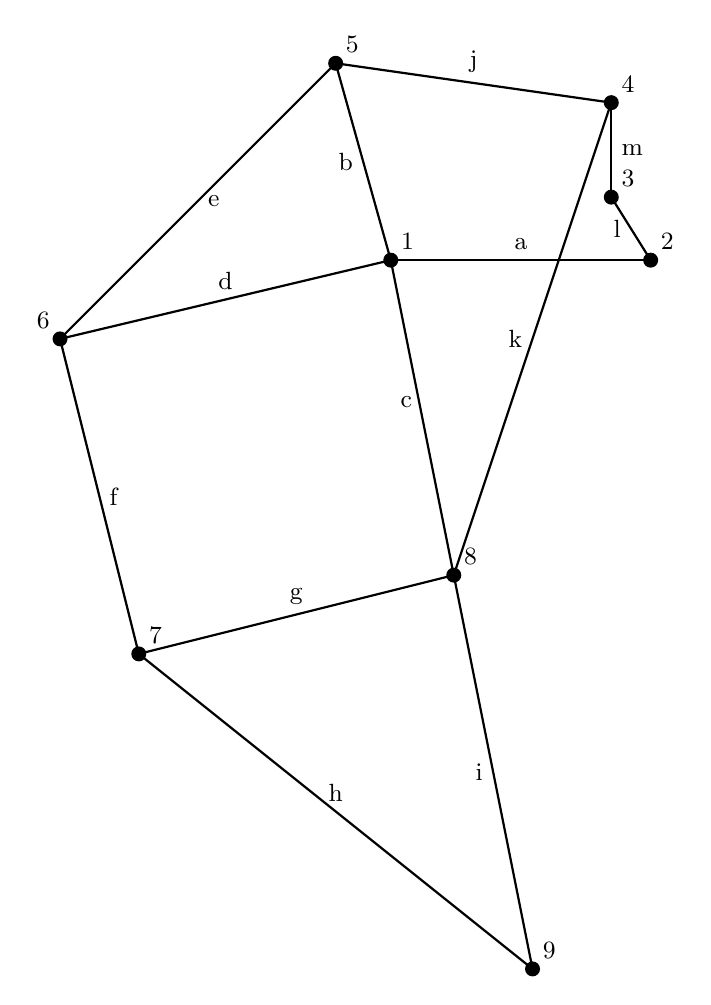
\begin{tikzpicture}[scale=0.1, thick, every node/.style={scale=1}]

  \coordinate (P1) at (22,30);
  \coordinate (P2) at (55,30);
  \coordinate (P3) at (50,38);
  \coordinate (P4) at (50,50);
  \coordinate (P5) at (15,55);
  \coordinate (P6) at (-20,20);
  \coordinate (P7) at (-10,-20);
  \coordinate (P8) at (30,-10);
  \coordinate (P9) at (40,-60);

  \draw (P1) -- (P2) node[midway,above] {\small a};
  \draw (P2) -- (P3) node[midway,left] {\small l};
  \draw (P3) -- (P4) node[midway,right] {\small m};
  \draw (P4) -- (P5) node[midway,above] {\small j};
  \draw (P5) -- (P1) node[midway,left] {\small b};
  \draw (P5) -- (P6) node[midway,right] {\small e};
  \draw (P6) -- (P1) node[midway,above] {\small d};
  \draw (P6) -- (P7) node[midway,right] {\small f};
  \draw (P1) -- (P8) node[midway,above left] {\small c};
  \draw (P7) -- (P8) node[midway,above] {\small g};
  \draw (P7) -- (P9) node[midway,above] {\small h};
  \draw (P9) -- (P8) node[midway,left] {\small i};
  \draw (P8) -- (P4) node[midway,left] {\small k};
  
  \filldraw (P1) circle (23pt) node[above right] {\small 1};
  \filldraw (P2) circle (23pt) node[above right] {\small 2};
  \filldraw (P3) circle (23pt) node[above right] {\small 3};
  \filldraw (P4) circle (23pt) node[above right] {\small 4};
  \filldraw (P5) circle (23pt) node[above right] {\small 5};
  \filldraw (P6) circle (23pt) node[above left] {\small 6};
  \filldraw (P7) circle (23pt) node[above right] {\small 7};
  \filldraw (P8) circle (23pt) node[above right] {\small 8};
  \filldraw (P9) circle (23pt) node[above right] {\small 9};
  \end{tikzpicture}
\end{figure}


\subsection{Materiales}

Dentro del marco del proyecto, se emplean diversos materiales para la construcción del mecanismo \textit{Theo Jansen}. Estos materiales son seleccionados fueron esocgidos por su durabilidad, flexibilidad y ligeresa, lo que permite que el mecanismo funcione de manera eficiente y efectiva. Los materiales utilizados incluyen:

\begin{itemize}
  \item \textbf{Sorbetes de plástico:} Estos sorbetes son utilizados para las patas del mecanismo, ya que son ligeros y flexibles, lo que permite que el mecanismo se mueva de manera eficiente. Además, los sorbetes son fáciles de conseguir y económicos, lo que los convierte en una opción ideal. Además de ser increíblemente resistentes ante la presión y torsión.
  
  \item \textbf{Hilo de coser o pavilo:} Este hilo se utiliza para unir las diferentes partes de la pata, hacen posible rotar a la articulación de manera que no es afectada por la fricción.
  
  \item \textbf{Palillos de manera:} Es importante fijar las patas a un eje central, para lo cual se utilizan palillos de madera. Estos palillos son resistentes y permiten unir las patas mediante el cigüeñal del mecanismo que convertirá el movimiento rotacional en movimiento lineal.1
  
\end{itemize}



